.%%%%%%%%%%%%%%%%%%%%%%%%%%%%%%%%%%%%%%%%%%%%%%%%%%%%
% Artifact Appendix Template for EuroSys'22 AE
%
% this document has a maximum length of 2 pages.
%%%%%%%%%%%%%%%%%%%%%%%%%%%%%%%%%%%%%%%%%%%%%%%%%%%%

% \appendix
%%%%%%%%%%%%%%%%%%%%%%%%%%%%%%%%%%%%%%%%%%%%%%%%%%%%%%%%%%%%%%%%%%%%%

\section{Artifact Appendix}
\label{sec:artifact}
\begin{tcolorbox}[colback=blue!5!white,colframe=blue!75!black]
\textbf{DOI:} \url{doi:10.5281/zenodo.6360540} \\
\textbf{Code:} \url{https://github.com/softsys4ai/unicorn}
\end{tcolorbox}

This appendix provides additional information regarding the tool that we have developed for evaluating \ourapproach. In this section, we call this tool \ourtool. In addition, we describe the steps using our \ourtool to reproduce the results reported in \S\ref{sec:effectiveness}, \S\ref{sec:transfer}, and \S\ref{sec:scalability}. We provide the source code and data in a publicly accessible GitHub repository that can be tested on any hardware once the software dependencies are met. 

\subsection{Description}
\ourapproach is used for performing tasks such as performance optimization and performance debugging in both offline and online modes. 
\begin{itemize}
    \item In the offline mode, \ourtool can be run on any device that uses previously measured configurations.
    \item In the online mode, the performance metrics are measured directly on the hardware on which the underlying configurable system is deployed, while the experiments are running. In the experiments, we have used \txtwo and \xavier. To collect measurements from these devices, \emph{sudo} privilege is needed, as it requires setting a device to a new configuration before measurement.
\end{itemize}
%  In both offline and online modes, \ourtool can be used for debugging and optimization for objectives such as latency and energy. 
 
%  \ourapproach has been implemented on six software systems such as \textsc{Deepstream} (Deepstream), \textsc{Xception} (Image), \textsc{Bert} (NLP), \textsc{Deepspeech} (Speech), \textsc{x264} (x264), and \textsc{sqlite} (sqlite).

% \subsection{Access}
% Our repository can be accessed online with the following link: \href{unicorn}{https://github.com/softsys4ai/unicorn}.

\subsection{Setup}


% \begin{tcolorbox}[colback=blue!5!white,colframe=blue!75!black]
% \textsc{NVIDIA Jetson Xavier}
%   \tcblower
% \textsc{Processor}: 6-core ARM CPU, 8 MB L2 + 4 MB L3

% \textsc{GPU}: 384-core Volta GPU with 48 Tensor cores

% \textsc{Memory}: 8 GB 256-bit LPDDR4x 1333MHz

% \textsc{Jetpack}: 4.3 \textsc{OS}: Ubuntu 20.04 64-bit
% \end{tcolorbox}
% \begin{tcolorbox}[colback=blue!5!white,colframe=blue!75!black]
% \textsc{NVIDIA Jetson TX2}
% \tcblower
% \textsc{Processor}: Dual-core NVIDIA Denver 2 64-bit CPU and quad-core Arm Cortex-A57 

% \textsc{GPU}: NVIDIA Pascal arch. with 256 CUDA cores

% \textsc{Memory}: 4 GB 128-bit LPDDR4 51.2 GB/s

% \textsc{Jetpack}: 4.3 \textsc{OS}: Ubuntu 20.04 64-bit
% \end{tcolorbox}

\subsubsection{Software Dependencies}
\ourtool is implement-ed by integrating and building on top of several existing tools (see \fig{unicorn-toolchain}): 
\begin{itemize}
    \item \href{https://semopy.com/}{\color{blue!80}semopy} for predictions with causal models.
    \item \href{https://ananke.readthedocs.io/en/latest/}{\color{blue!80}ananke} and \href{https://github.com/akelleh/causality}{\color{blue!80}causality} for estimating the causal effects.
    \item \href{https://github.com/cmu-phil/causal-learn}{\color{blue!80}causal-learn} for structure learning. 
\end{itemize}


\subsubsection{Hardware Dependencies}
\ourtool is implemented both in offline and online modes. There are no particular hardware dependencies to run \ourtool in offline mode. To run \ourtool in online mode, we used hardware that has sensors for performance measurements. In particular, we used \txone, \txtwo, and \xavier with \emph{Jetpack 4.3} and \emph{Ubuntu 20.04 LTS}.

\subsubsection{Installation}
We use \textit{docker-compose} to install the necessary software required to run \ourtool. The necessary steps to install the dependencies and third-party libraries used to test our approach can be done with the following commands.

\begin{verbatim}
git clone git@github.com:softsys4ai/unicorn.git
cd unicorn
docker-compose up --build --detach
\end{verbatim}


\begin{figure}[hb!]
    \centering
    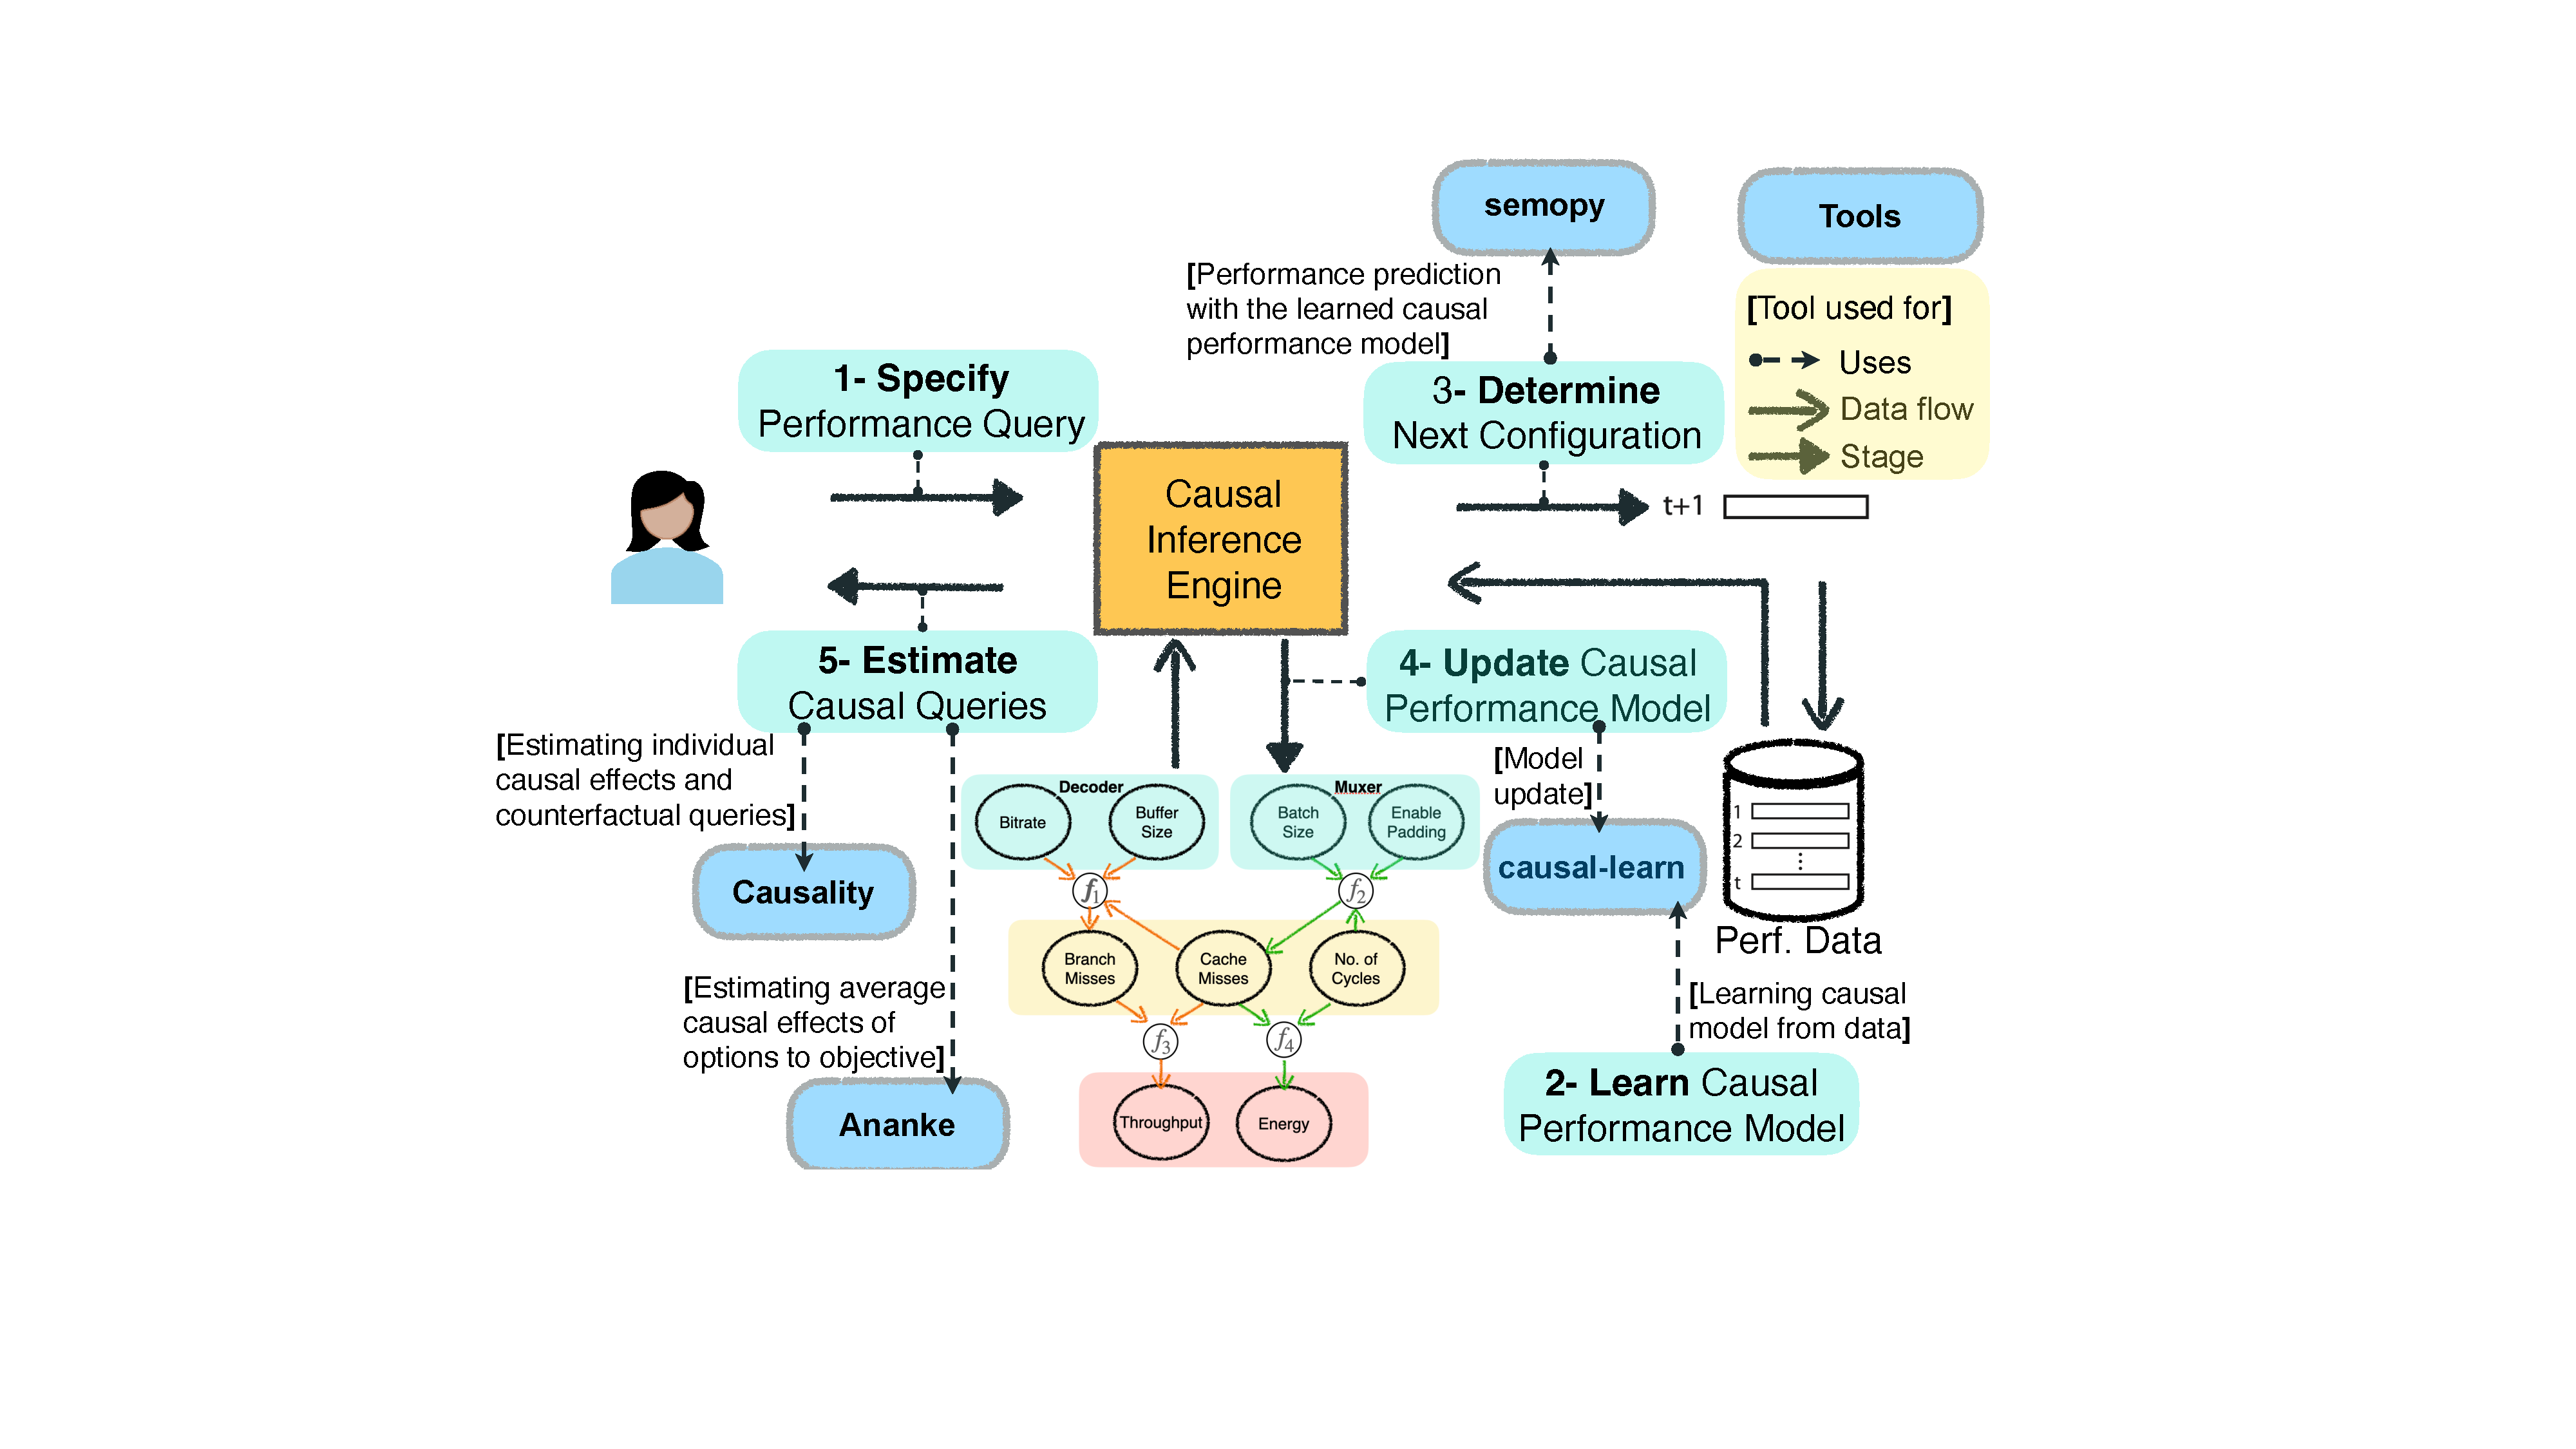
\includegraphics[width=\linewidth]{figures-vg/UnicornTool.pdf}
    \caption{Toolchain in \ourtool.}
    \label{fig:unicorn-toolchain}
\end{figure}

Once this step is completed, \ourtool is ready to be tested.


\subsection{Data} 
All the datasets required to run experiments are already included in the \textit{./unicorn/data} directory.  

\subsection{Major Claims}
We make the following major claims in our paper:
\begin{itemize}
\item \ourapproach can be used to detect root causes of non-functional performance (latency and energy) faults with higher accuracy and gain.

\item \ourapproach can support performing downstream performance tasks such as performance optimization.

\item The causal performance models are transferable across environments (different workload or hardware) and can be efficiently re-used from the source environment where it is trained to a target environment.
\end{itemize}

\subsection{Experiments}
We run the following experiments to support our claims.

\subsubsection{E1: Performance Debugging Experiment} To support the claim of efficiency of \ourapproach in debugging non-functional faults, we reproduce energy faults results for \textsc{Xception} in \textsc{Nvidia Jeston Xavier} from Table~\ref{tab:single_1}. Our initial study discovered 29 energy faults for \textsc{Xception} in \textsc{Nvidia Jetson Xavier,} that is 12\% of the faults reported in Table~\ref{tab:single_1}. This would require ~1.5 hours to run the experiments in offline mode and ~11 hours to run the experiments in online mode.

\noindent\textbf{Execution}. To run \ourtool on a single bug, execute the following command:

\begin{verbatim}
docker-compose exec unicorn python \\ 
./tests/run_unicorn_debug.py -o \\
total_energy_consumption -s Image -k Xavier \\
-m offline\online -i 0
\end{verbatim}

To run \ourtool and other debugging baselines reported in this paper on all the bugs, please use the following commands one by one:
\begin{verbatim}
docker-compose exec unicorn python \\ 
./tests/run_unicorn_debug.py -o \\
total_energy_consumption -s Image -k Xavier \\
-m offline\online 
    
docker-compose exec unicorn python \\ 
./tests/run_baseline_debug.py -o \\
total_energy_consumption -s Image -k Xavier \\
-m offline\online -b cbi 
    
docker-compose exec unicorn python \\ 
./tests/run_baseline_debug.py -o \\
total_energy_consumption -s Image -k Xavier \\
-m offline\online -b encore
    
docker-compose exec unicorn python \\ 
./tests/run_baseline_debug.py -o \\
total_energy_consumption -s Image -k Xavier \\
-m offline\online -b bugdoc
    
\end{verbatim}

\noindent \textbf{Results}. We save the evaluation metrics such as accuracy, precision, recall, gain, and time required for debugging. A separate plot is generated using the recommended fixes to compare \ourapproach with other baseline approaches with their evaluation metrics. Note, in the offline mode the reported time is different (usually less) from the main text as instead of running the measurements online we reuse recorded measurements. However, we can get a sense of the efficiency by comparing the number of samples required to resolve a fault.

\subsubsection{E2: Performance Optimization Experiment} \ourapproach supports can support performing downstream performance tasks such as performance optimization. To support this claim, we reproduce single-objective latency optimization results reported in \fig{rq1_opt_se} (a). This experiment would require around ~1.5 hours to complete in the offline mode and ~4 hours to complete in the online mode. We also compare the results with a baseline optimization approach, \textsc{SMAC}, reported in the paper. 


\noindent \textbf{Execution}. To run the experiment, we need to execute the following commands:

\begin{verbatim}
docker-compose exec unicorn python \\ 
./tests/run_unicorn_optimization.py -o \\
inference_time -s Image -k TX2 \\
-m offline\online 
    
docker-compose exec unicorn python \\ 
./tests/run_baseline_optimization.py -o \\
inference_time -s Image -k TX2 \\
-m offline\online -b smac
\end{verbatim}

\noindent \textbf{Results}. We display the results similar to \fig{rq1_opt_se} (a) using a line plot. Note that this experiment is run once without repeating, so there are no error bars.

\subsubsection{E3: Transferability Experiment.} To support this claim, we initially build a causal performance model to resolve the latency faults in \xavier and reuse the causal performance model to resolve the latency faults in \txtwo. We only use one bug to demonstrate this result. This would require ~10 minutes to run the experiment in the offline mode and ~25 minutes in the online mode. 

\noindent \textbf{Execution}. The following command runs the experiments:

\begin{verbatim}
docker-compose exec unicorn python \\ 
./tests/run_unicorn_transferability.py -o \\
inference_time -s Image -k Xavier \\
-m offline\online 

\end{verbatim}

\noindent \textbf{Results}. The evaluation metrics, including accuracy, precision, recall, gain, and time required for debugging for different scenarios reported in the paper are saved to a separate CSV file after the experiments are over and plotted. Note that the reported time is different from the time reported in the main text in the offline mode. 

\subsection{Using \ourtool with external data}
We added \href{https://github.com/softsys4ai/unicorn/blob/master/artifact/OTHERS.md}{\color{blue!80}instructions} to describe the required steps to use \ourtool with any other external dataset.

\subsection{Extending \ourtool}
We welcome any contribution for extending either \ourapproach (see \S\ref{sec:discussion} for several possible future directions) and \ourtool for performance improvements or feature extensions.  


%%%%%%%%%%%%%%%%%%%%%%%%%%%%%%%%%%%%%%%%%%%%%%%%%%%%%%%%%%%%%%%%%%%%%